\documentclass[utf8, 11pt]{beamer}
\usepackage{verbatim}
\usepackage{color}
\usepackage{graphicx}
\usepackage{alltt}
%\usepackage{hyperref}
%\hypersetup{colorlinks=true, urlcolor=cyan}
\hypersetup{urlcolor=cyan}

\mode<presentation>
{
  \usetheme{default}
}

\usepackage[english, russian]{babel}
\usepackage{graphicx}
\usepackage{colortbl}
\usepackage{listings}

\newcommand{\rsb}{\cellcolor[gray]{0.85}}
\newcommand{\nam}[1]{\texttt{#1}}

\setbeamertemplate{navigation symbols}{} 

\author[ ]{Карташов Д. А.}

\title[Virtual HSM]{Разработка виртуального HSM}

\institute[СПбАУ]
{
  Кафедра математических и информационных технологий\\
  Санкт-Петербургский Академический университет
}

\date{ }

\subject{Talks}

\useoutertheme{infolines}
\setbeamertemplate{headline}{}

\begin{document}

\begin{frame}
  \titlepage
\end{frame}

\begin{frame}{Введение}

Криптография в приложениях:
\begin{itemize}
\item хранение секретных данных
\item вычисления с их использованием
\end{itemize}

\vspace*{\fill}

Проблемы безопасности:
\begin{itemize}
\item компрометация секретных данных
\end{itemize}

\vspace*{\fill}

Решение:
\begin{itemize}
\item исключить попадание секретных данных на диск и/или в память компьютера
\end{itemize}

\vspace*{\fill}

Цель проекта:
\begin{itemize}
\item разработка решения, предоставляющего функциональность HSM в виртуальном окружении
\end{itemize}

\end{frame}

\begin{frame}{Общая архитектура решения}
\begin{center}
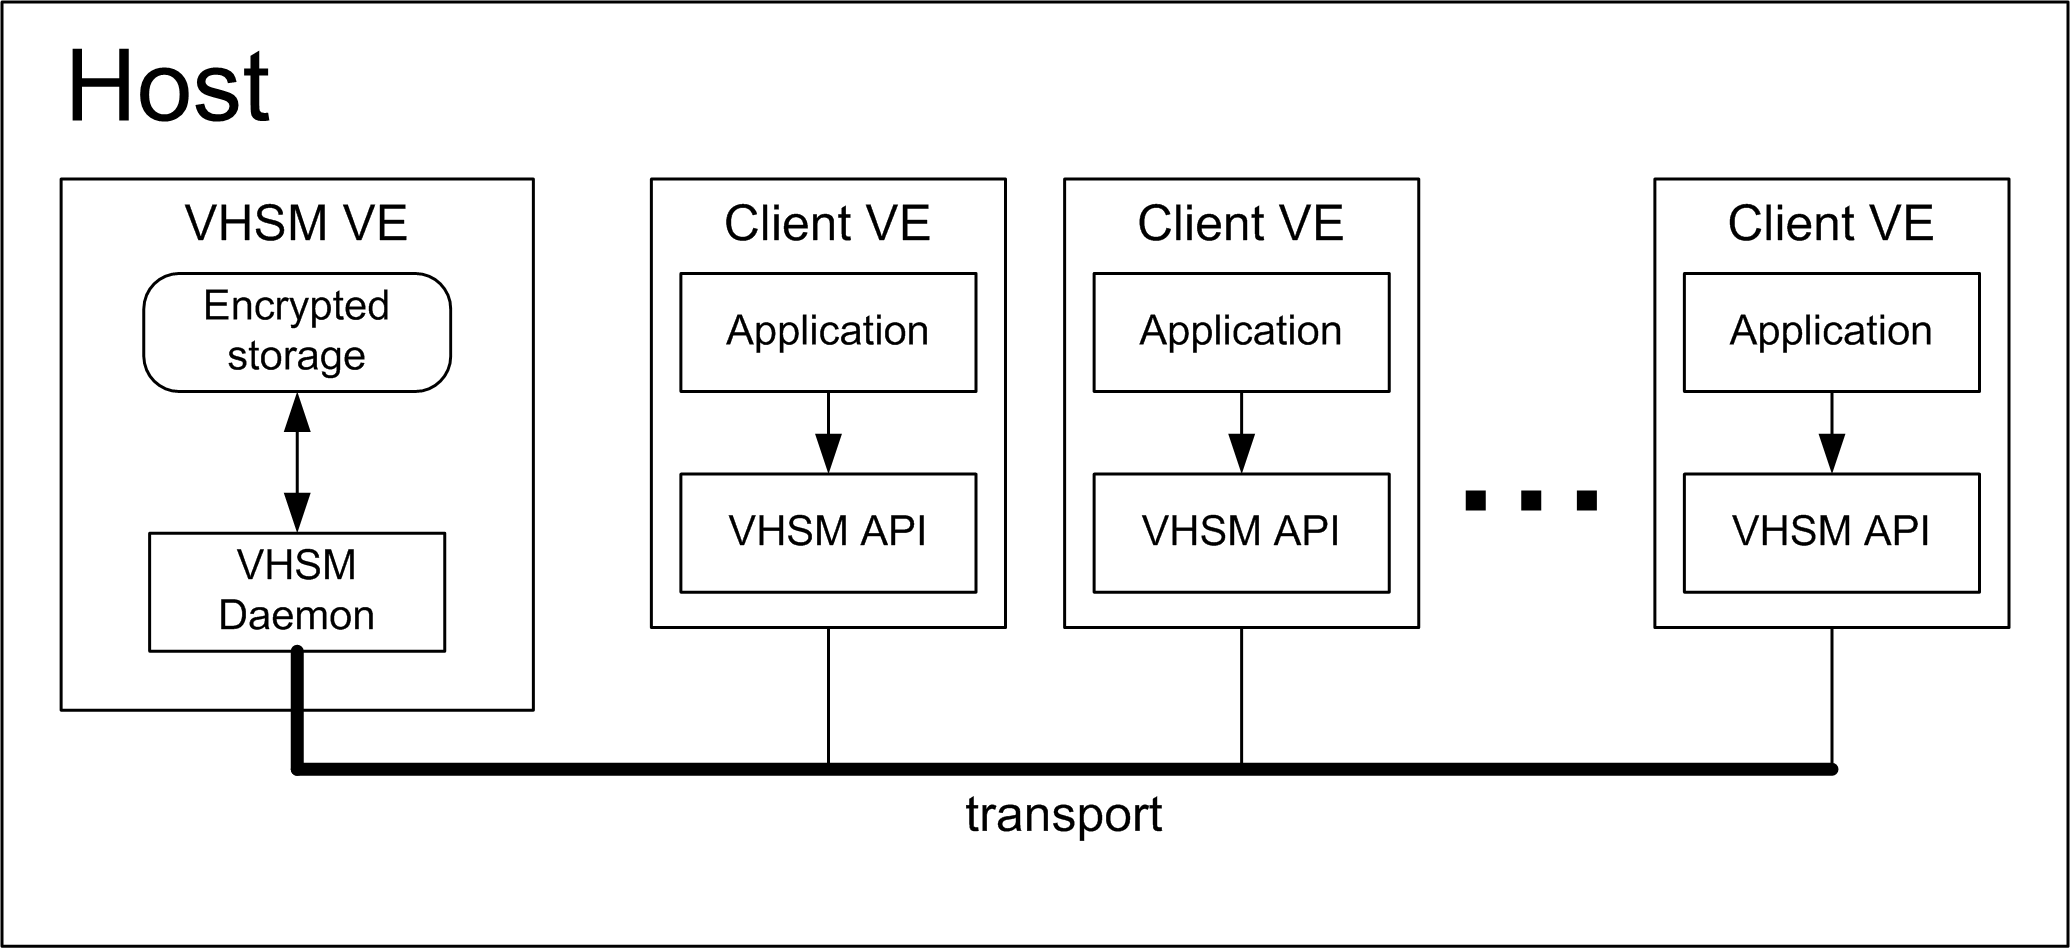
\includegraphics[width=0.94\paperwidth]{img2}
\end{center}
\end{frame}

\begin{frame}{Основные компоненты}
\begin{itemize}
\item {\bf VHSM server}
	\begin{itemize}
		\item аутентификация
		\item выполнение криптографических операций с использованием секретных данных
	\end{itemize}
\item {\bf Encrypted storage}
	\begin{itemize}
		\item хранение секретных данных пользователя
	\end{itemize}
\item {\bf VHSM API}
	\begin{itemize}
		\item передача запросов на выполнение операций через транспорт
		\item получение результатов операций
	\end{itemize}
\item {\bf Transport}
	\begin{itemize}
		\item пересылка сообщений
		\item идентификация контейнеров
	\end{itemize}
\item {\bf OpenSSL engine}
	\begin{itemize}
		\item интерфейс между VHSM API и пользовательским приложением
	\end{itemize}
\end{itemize}

\end{frame}

\begin{frame}{VHSM server \& encrypted storage}

\begin{itemize}
\item доступ:
\begin{itemize}
	\item логин и пароль пользователя;
	\item на основе пароля функцией PBKDF2 генерируется мастер-ключ шифрования данных пользователя;
\end{itemize}

\item аутентификация:
\begin{itemize}
	\item 256-битный ключ аутентификации, зашифрованный с помощью мастер-ключа в режиме GCM;
\end{itemize}

\item вычисление криптографических функций:
\begin{itemize}
	\item обращение к секретным данным по их идентификатору;
	\item пользователью возвращается только результат операции;
\end{itemize}

\item хранение секретных данных:
\begin{itemize}
	\item база данных SQLite;
\end{itemize}
\end{itemize}

\vspace*{\fill}

\end{frame}

\begin{frame}{VHSM API}

\begin{itemize}
\item управление сессиями
\begin{itemize}
\item открытие/завершение сессии;
\item аутентификация пользователя;
\end{itemize}

\item управление ключами
\begin{itemize}
\item импорт;
\item генерация;
\item удаление;
\end{itemize}

\item хэширование и МАС
\begin{itemize}
\item стандартные функции: \texttt{init, update, final}
\end{itemize}
\end{itemize}

\vspace*{\fill}

\end{frame}

\begin{frame}[fragile]
\frametitle{Transport}
\begin{itemize}
\item протокол --- \texttt{Google Protobuf}
\item реализован на основе netlink
\end{itemize}
\begin{center}
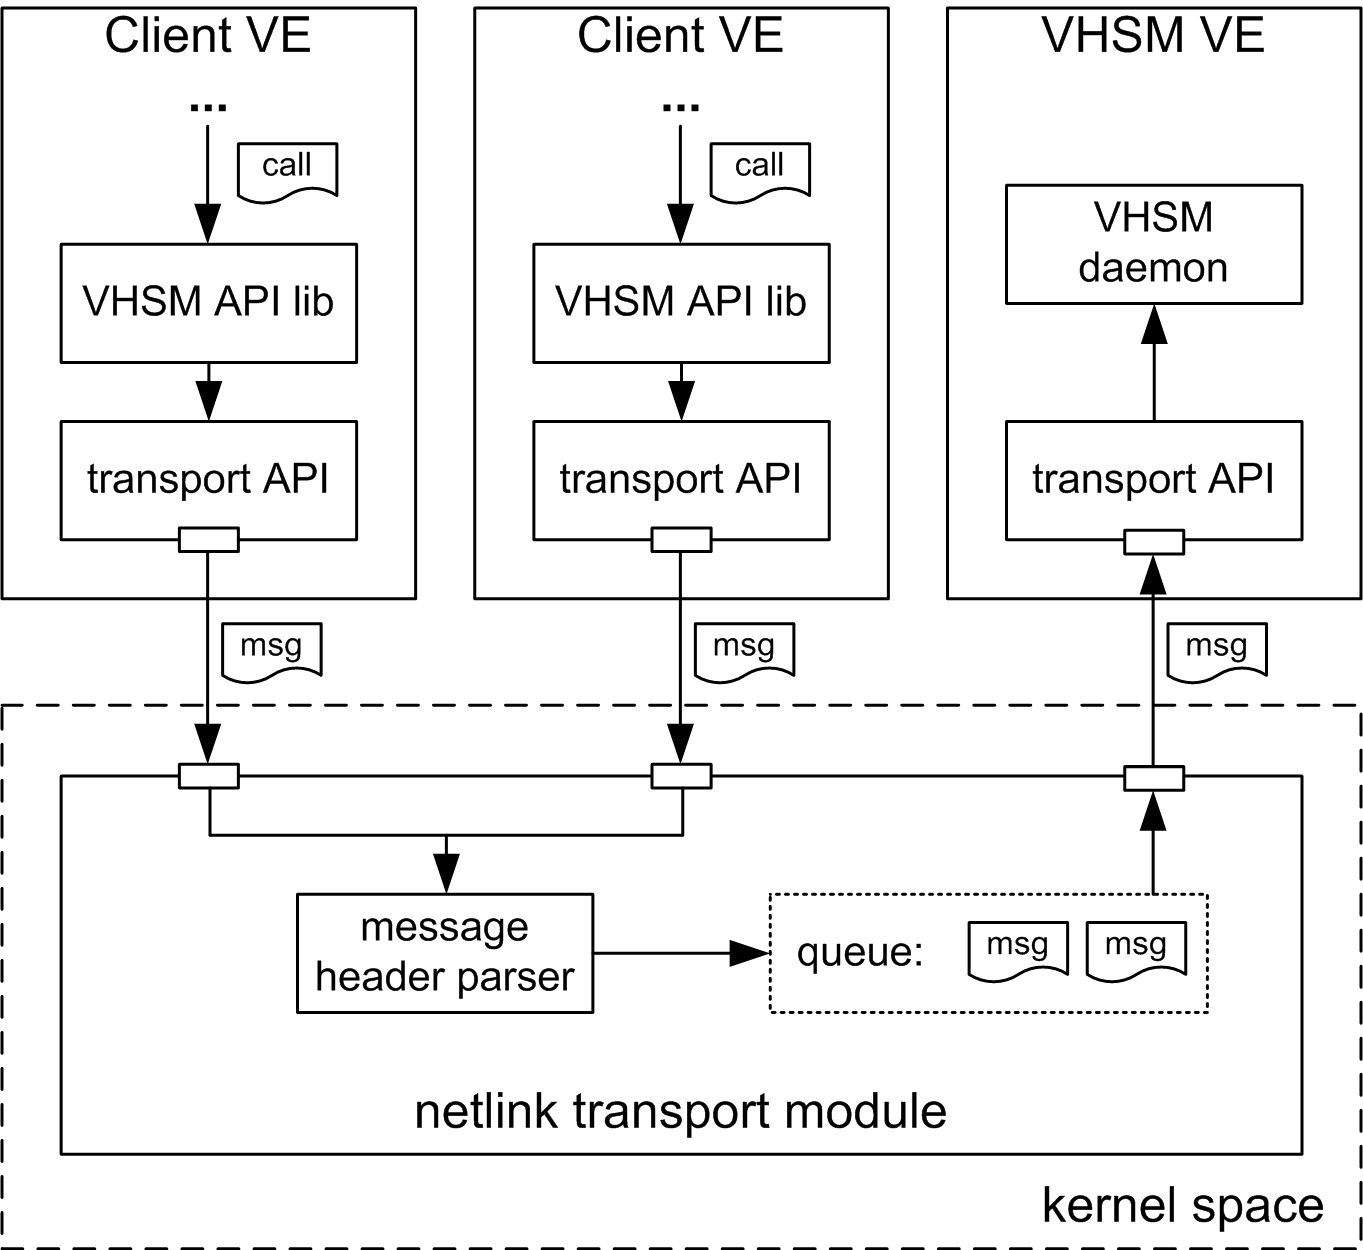
\includegraphics[scale=0.65]{img4-1}
\end{center}
\end{frame}

\begin{frame}{OpenSSL engine}

{\bf OpenSSL engine} может быть использован для делегирования криптографических функций VHSM.

\vspace*{\fill}

В текущей реализации изменен алгоритм хэширования, что позволяет использовать стандартные функции для HMAC.

\vspace*{\fill}

Минусы:
\begin{itemize} 
\item алгоритм работы движка опирается на текущую реализацию функций в OpenSSL;
\item возможная уязвимость при использовании конфигурационных файлов;
\end{itemize}

Плюсы:
\begin{itemize}
\item от конечного пользователя требуется меньше усилий для внедрения поддержки VHSM в свое приложение.
\end{itemize}

\vspace*{\fill}

\end{frame}

\begin{frame}{Пример использования}
\begin{center}
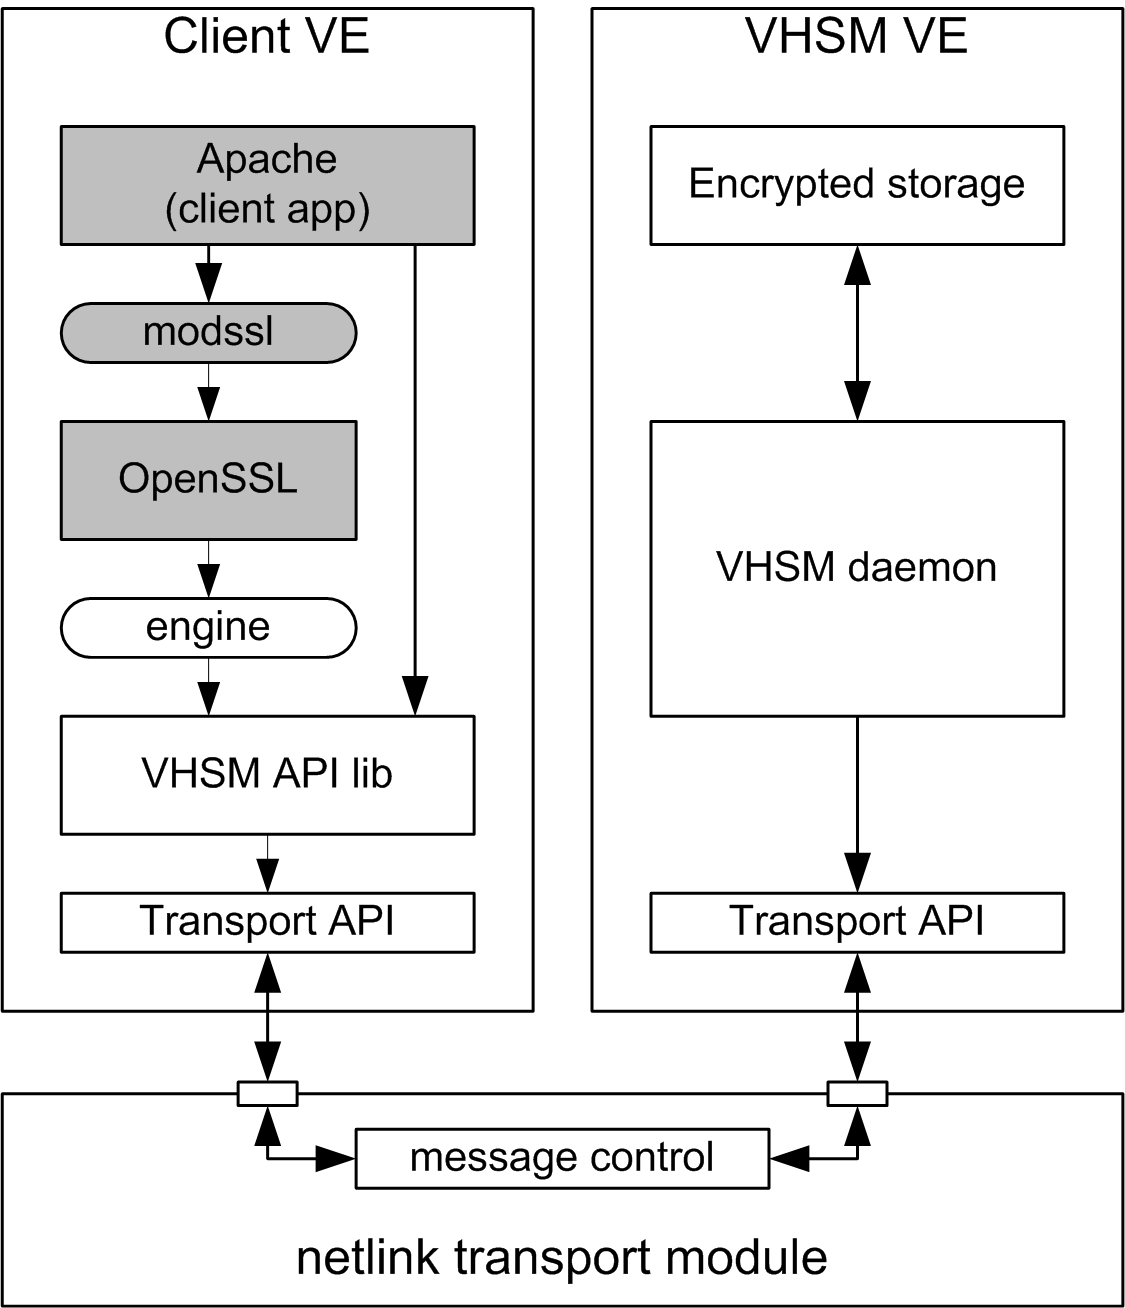
\includegraphics[scale=0.70]{img3-3}
\end{center}
\end{frame}

\begin{frame}{Итоги}

Возможные направления развития проекта:
\begin{itemize}
\item введение ролей пользователей и уровней доступа к VHSM и хранилищу;
\item расширение функциональности VHSM;
\item адаптация для других виртуальных окружений.
\end{itemize}

\vspace*{\fill}

Ссылки:
\begin{itemize}
\item репозиторий:

\url{https://github.com/OSLL/vhsm}

\item баг-трекер:

\url{http://dev.osll.ru/projects/vhsm}
\end{itemize}

\vspace*{\fill}

\end{frame}

\end{document}
